\begin{enumerate}[label=\thesection.\arabic*,ref=\thesection.\theenumi]
\item Show that
\begin{equation}
    \frac{1\times2^2 + 2\times3^2 + \dots + n\times\brak{n+1}^2}{1^2\times2 + 2^2\times3 +\dots + n^2\times\brak{n+1}}  = \frac{3n+5}{3n+1}\notag
\end{equation}

\solution 

\iffalse
\let\negmedspace\undefined
\let\negthickspace\undefined
\documentclass[journal,12pt,twocolumn]{IEEEtran}
\usepackage{cite}
\usepackage{amsmath,enumitem,amssymb,amsfonts,amsthm}
\usepackage{algorithmic}
\usepackage{graphicx}
\usepackage{float}
\usepackage{textcomp}
\usepackage{xcolor}
\usepackage{caption}
\usepackage{txfonts}
\usepackage{listings}
\usepackage{enumitem}
\usepackage{mathtools}
\usepackage{gensymb}
\usepackage{comment}
\usepackage[breaklinks=true]{hyperref} 
\usepackage{tkz-euclide} 
\usepackage{listings}
\usepackage{tabularx}
\usepackage{gvv}                                        
\def\inputGnumericTable{}                                 
\usepackage[latin1]{inputenc}                              
\usepackage{color}                                            
\usepackage{array}                                            
\usepackage{longtable}                                       
\usepackage{calc}                                             
\usepackage{multirow}                                         
\usepackage{hhline}                                           
\usepackage{ifthen}                                        
\usepackage{lscape}
\newtheorem{theorem}{Theorem}[section]
\newtheorem{problem}{Problem}
\newtheorem{proposition}{Proposition}[section]
\newtheorem{lemma}{Lemma}[section]
\newtheorem{corollary}[theorem]{Corollary}
\newtheorem{example}{Example}[section]
\newtheorem{definition}[problem]{Definition}
\newcommand{\BEQA}{\begin{eqnarray}}
\newcommand{\EEQA}{\end{eqnarray}}
\newcommand{\define}{\stackrel{\triangle}{=}}
\theoremstyle{remark}
\newtheorem{rem}{Remark}
\begin{document}
\bibliographystyle{IEEEtran}
\vspace{3cm}
\title{NCERT 11.9.5 26Q}
\author{EE23BTECH11015 - DHANUSH V NAYAK$^{*}$% <-this % stops a space
}
\maketitle
\newpage
\bigskip
\renewcommand{\thefigure}{\arabic{figure}}
\renewcommand{\thetable}{\theenumi}
\bibliographystyle{IEEEtran}
\textbf{\underline{RESULTS AND DERIVATIONS}}

\newpage
\textbf{Question:} Show that
\begin{equation}
    \frac{1\times2^2 + 2\times3^2 + \dots + n\times\brak{n+1}^2}{1^2\times2 + 2^2\times3 +\dots + n^2\times\brak{n+1}}  = \frac{3n+5}{3n+1}\notag
\end{equation}
\textbf{Solution:}
\fi 

\begin{table}[h]
    \centering
    \renewcommand\thetable{1}
    \setlength{\extrarowheight}{9pt}
    \resizebox{0.54\textwidth}{!}{
    \begin{tabular}{|c|c|c|}
    \hline
    \textbf{Parameter} & \textbf{Description} & \textbf{Value} \\ \hline
    $n$ & Integer &.... -2,-1,0,1, 2, ... \\ \hline
    $x_1(n)$ & General term of Numerator & $\vphantom{\brak{n^{3}}} \brak{n^{3} + 5n^{2} + 8n + 4} \cdot u\brak{n}$ \\ \hline
    $x_2(n)$ & General Term of Denominator  & $\vphantom{\brak{n^{3}}} \brak{n^{3}+4n^{2}+5n+2}\cdot u\brak{n}$ \\ \hline
    $y_1\brak{n}$ & Sum of terms of numerator & $?$ \\ \hline
    $y_2\brak{n}$ & Sum of terms of denominator & $? $ \\ \hline
    $U(z)$ & z-transform of $u(n)$ & $\frac{1}{1 - z^{-1}\vphantom {\brak{0.3pt}}},\cbrak{z\in\mathbb{C} : \lvert z \rvert > 1}$ \\ \hline 
    ROC & Region of convergence & $\left\{ z : \left|\sum_{n=-\infty}^{\infty} x(n)z^{-n}\right| < \infty \vphantom {\brak{{0.3pt}}}\right\}$ \\ \hline 
    \end{tabular}}
    \caption{Parameter Table}
    \label{tab:11.9.5.26.1}
    \end{table}
    
    
    
    
\begin{enumerate}[label=\arabic*.]
\item \underline {Analysis of Numerator:}\\
\begin{align}
 X_1\brak{z} &= \sum_{n=-\infty}^\infty x_1\brak{n}  z^{-n}\\
             &= \sum_{n=-\infty}^\infty \brak{n^{3} + 5n^{2} + 8n + 4} u\brak{n} z^{-n}
\end{align}
Using results of equations \eqref{eq:11.9.5.26.2} to \eqref{eq:11.9.5.26.5} we get:
\begin{align}
 \therefore   X_1\brak{z}&= \frac{4+2z^{-1}}{\brak{1-z^{-1}}^4} ,   \abs{z} >1 
\end{align}
From \eqref{eq:conv-sum}
\begin{align}
y_1\brak{n} &= x_1\brak{n}\ast u\brak{n}\\
    Y_1\brak{z} &= X_1\brak{z} U\brak{z} \\
 &= \frac{4+2z^{-1}}{\brak{1-z^{-1}}^5} , \abs{z}> 1 
\end{align}
Using partial fractions:
\begin{align}
    Y_1(z) &= \frac{22z^{-1}}{\brak{1-z^{-1}}} + \frac{48z^{-2}}{\brak{1-z^{-1}}^2} + \frac{52z^{-3}}{\brak{1-z^{-3}}^3} , \label{eq:11.9.5.26.6}\\
    &+ \frac{28z^{-4}}{\brak{1-z^{-1}}^4}+\frac{6z^{-5}}{\brak{1-z^{-1}}^5}+4 , \abs{z}>1 \notag 
\end{align}
Substituting results of equation \eqref{eq:11.9.5.26.9} to \eqref{eq:11.9.5.26.12} in equation \eqref{eq:11.9.5.26.6}:
\begin{align}
    y_1\brak{n} &= \frac{3n^4 + 26n^3 + 81n^2 + 106n + 48}{12}u\brak{n}\\
    &= \frac{\brak{3n+8}\brak{n+1}\brak{n+2}\brak{n+3}}{12}u\brak{n}
\end{align}
\item \underline{Analysis of Denominator:}
\begin{align}
    X_2\brak{z} &= \sum_{n=-\infty}^\infty x_2\brak{n} z^{-n}\\
                &= \sum_{n=-\infty}^\infty \brak{n^{3}+4n^{2}+5n+2} u\brak{n} z^{-n}
\end{align}
\text{Using results of equation \eqref{eq:11.9.5.26.2} to \eqref{eq:11.9.5.26.5} we get:}
\begin{align}
   \therefore  X_2\brak{z} &= \frac{2+4z^{-1}}{\brak{1-z^{-1}}^4},   \abs{z} >1   
\end{align}
From \eqref{eq:conv-sum}
\begin{align}
    y_2\brak{n} &= x_2\brak{n}\ast u\brak{n}\\
    Y_2\brak{z} &= X_2\brak{z} U\brak{z} \\
 &=\frac{2+4z^{-1}}{\brak{1-z^{-1}}^5} ,   \abs{z} >1 
\end{align}
Using partial fractions:
\begin{align}
    Y_2\brak{z} &= \frac{14z^{-1}}{\brak{1-z^{-1}}} + \frac{36z^{-2}}{\brak{1-z^{-1}}^2} + \frac{44z^{-3}}{\brak{1-z^{-3}}^3} \label{eq:11.9.5.26.13}\\
    &+ \frac{26z^{-4}}{\brak{1-z^{-1}}^4}+\frac{6z^{-5}}{\brak{1-z^{-1}}^5}+2 , \abs{z}>1\notag 
\end{align}
Substituting results of equation \eqref{eq:11.9.5.26.9} to \eqref{eq:11.9.5.26.12} in equation \eqref{eq:11.9.5.26.13}:
\begin{align}
    y_2\brak{n} &=  \frac{3n^4 + 22n^3 + 57n^2 + 62n + 24}{12}u\brak{n}\\
                &= \frac{\brak{3n+4}\brak{n+1}\brak{n+2}\brak{n+3}}{12}u\brak{n}
\end{align}
As the sequence start from $n=0$ , in RHS of question $n$ should be replaced by $n+1$:
\begin{align}
    \frac{y_1\brak{n}}{y_2\brak{n}} = \frac{3n+8}{3n+4}
\end{align}
Hence Prooved.
\end{enumerate}
\begin{figure}[htbp]
    \centering
    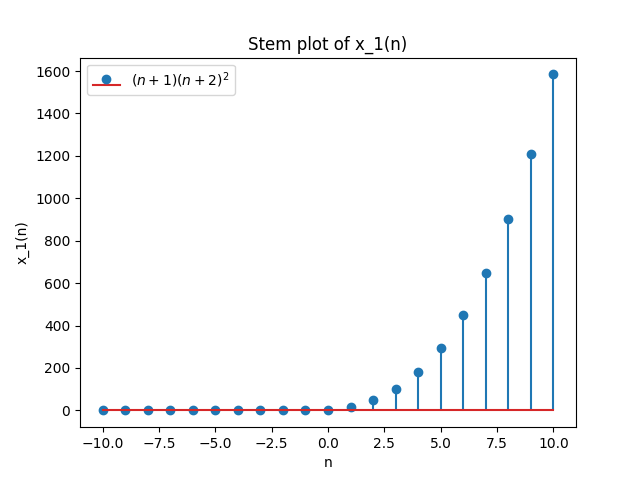
\includegraphics[width=1\columnwidth]{ncert-maths/11/9/5/26/figs/x1_plot.png}
    \caption{Stem Plot of $x_1\brak{n}$}
    \label{fig:x1}
\end{figure}
\begin{figure}[htbp]
    \centering
    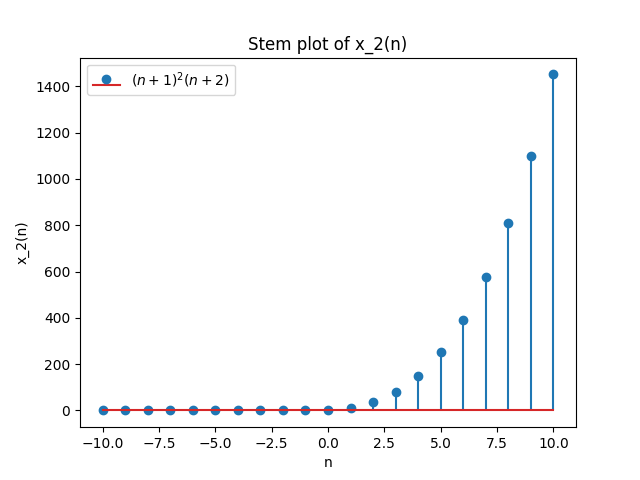
\includegraphics[width=1\columnwidth]{ncert-maths/11/9/5/26/figs/x2_plot.png}
    \caption{Stem Plot of $x_2\brak{n}$}
    \label{fig:x2}
\end{figure}
\begin{figure}[htbp]
    \centering
    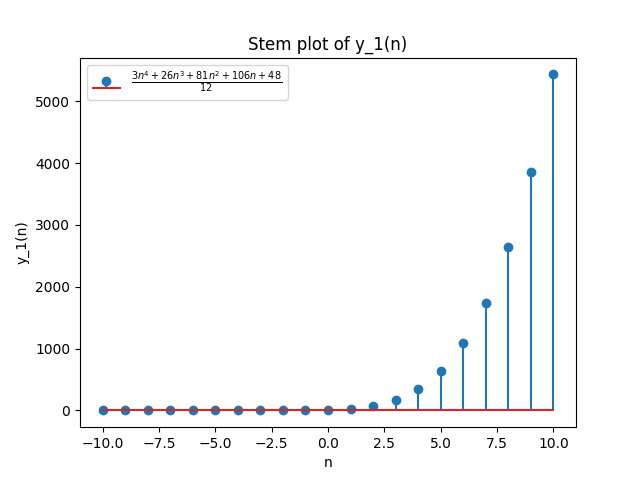
\includegraphics[width=1\columnwidth]{ncert-maths/11/9/5/26/figs/y1_plot.png}
    \caption{Stem Plot of $y_1\brak{n}$}
    \label{fig:y1}
\end{figure}
\begin{figure}[h]
    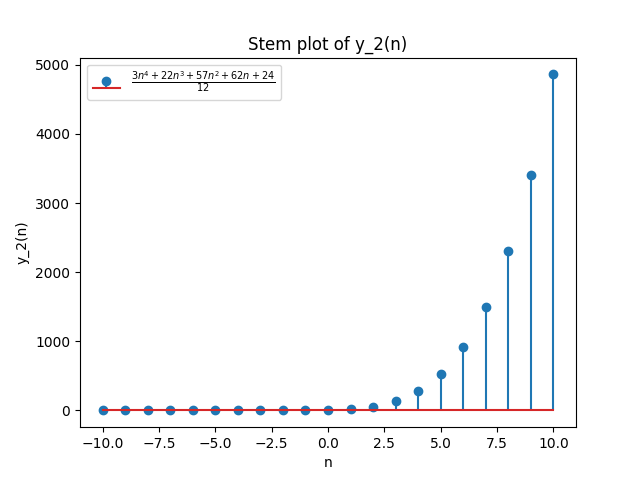
\includegraphics[width=1\columnwidth]{ncert-maths/11/9/5/26/figs/y2_plot.png}
    \caption{Stem Plot of $y_2\brak{n}$}
    \label{fig:y2}
\end{figure}
%\end{document}

\pagebreak

\item Write the five terms at n = 1, 2, 3, 4, 5 of the sequence and obtain the Z-transform of the series
\begin{align}
    x \brak{n} &=  -1, & n = 0 \\
    &=   \frac{x \brak{n-1}}{n}, & n > 0\\
    &=   0, & n < 0 
\end{align}

\solution

\iffalse
\let\negmedspace\undefined
\let\negthickspace\undefined
\documentclass[journal,12pt,twocolumn]{IEEEtran}
\usepackage{cite}
\usepackage{amsmath,amssymb,amsfonts}
\usepackage{graphicx}
\usepackage{textcomp}
\usepackage{xcolor}
\usepackage{txfonts}
\usepackage{listings}
\usepackage{enumitem}
\usepackage{mathtools}
\usepackage{gensymb}
\usepackage{comment}
\usepackage[breaklinks=true]{hyperref}
\usepackage{tkz-euclide} 
\usepackage{listings}
\usepackage{gvv}                                        
\def\inputGnumericTable{}                                 
\usepackage[latin1]{inputenc}                                
\usepackage{color}                                            
\usepackage{array}                                            
\usepackage{longtable}                                       
\usepackage{calc}                                             
\usepackage{multirow}                                         
\usepackage{hhline}                                           
\usepackage{ifthen}                                           
\usepackage{lscape}
\usepackage[export]{adjustbox}

\newtheorem{theorem}{Theorem}[section]
\newtheorem{problem}{Problem}
\newtheorem{proposition}{Proposition}[section]
\newtheorem{lemma}{Lemma}[section]
\newtheorem{corollary}[theorem]{Corollary}
\newtheorem{example}{Example}[section]
\newtheorem{definition}[problem]{Definition}
\newcommand{\BEQA}{\begin{eqnarray}}
\newcommand{\EEQA}{\end{eqnarray}}
\newcommand{\define}{\stackrel{\triangle}{=}}
\newtheorem{rem}{Remark}

\begin{document}
\parindent 0px
\bibliographystyle{IEEEtran}

\vspace{3cm}

\title{}
\author{EE23BTECH11217 - Prajwal M$^{*}$
}
\maketitle
\newpage
\bigskip

 \renewcommand{\thefigure}{\theenumi}
 \renewcommand{\thetable}{\theenumi}


\section*{Exercise 9.1}

\noindent \textbf{12} \hspace{2pt}Write the five terms at n = 1, 2, 3, 4, 5 of the sequence and obtain the Z-transform of the series
\begin{align}
    x \brak{n} &=  -1, & n = 0 \\
    &=   \frac{x \brak{n-1}}{n}, & n > 0\\
    &=   0, & n < 0 
\end{align}

\noindent Solution:
\fi
\noindent
\begin{align}
	x \brak{1} & = \frac{x \brak{0}}{1} = -1 \\
x \brak{2} & = \frac{x \brak{1}}{2} = -\frac{1}{2} \\
	x \brak{3} & = \frac{x \brak{2}}{3} = -\frac{1}{\brak{2} \brak{3}} = -\frac{1}{6}\\
	x \brak{4} & = \frac{x \brak{3}}{4} = -\frac{1}{\brak{2}   \brak{3} \brak{4}} = -\frac{1}{24}\\
	x \brak{5} & = \frac{x \brak{4}}{5} = -\frac{1}{\brak{2} \brak{3} \brak{4} \brak{5}} = -\frac{1}{120} \\
    x \brak{n} & = \frac{-1}{n!}  \brak{u \brak{n}} \label{x(n)}
\end{align}
\begin{align}
	x \brak{n} & \system{Z} X \brak{z} 
\end{align}

\begin{figure}[h]
   \centering
   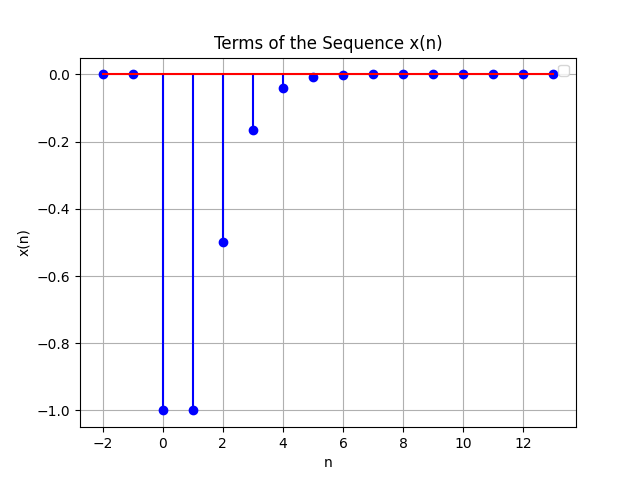
\includegraphics[width=1\columnwidth]{ncert-maths/11/9/1/12/figs/plot.png}
   \caption{Plot of x(n) vs n}
   \label{fig: 9.1.12.1}
\end{figure}

\begin{align}
    X \brak{z} & = \sum_{n=-\infty}^{\infty} x \brak{n}   z^{-n} \\
    \notag \text{using \eqref{x(n)}, } \\
    & = \sum_{n=-\infty}^{\infty} \frac{-1}{n!}  u \brak{n}   z^{-n} \\
    & = \sum_{n=0}^{\infty} \frac{-1}{n!}   z^{-n} \\
    & = - e^{z^{-1}} &  \cbrak{z\in\mathbb{C} : z \neq 0} 
\end{align}

\begin{table}[h]
    \centering
      \begin{tabular}{|c|c|c|}
    \hline
    	\textbf{Symbol} & \textbf{Value} & \textbf{Description} \\
    \hline
	  $x(n)$ & $\frac{-1}{n!}$ & general term of the series \\
    \hline
	  $X(z)$ & $- e^{z^{-1}}$ &Z-transform of x(n) \\
    \hline 
	  $u(n)$ & &unit step function \\
    \hline
  \end{tabular}

    \caption{Parameters}
    \label{tab: 9.1.12.1}
\end{table}


%\end{document}

\pagebreak


\item Subba Rao started work in 1995 at an annual salary of Rs. 5000 and received an increment of Rs. 200 each year. In which year did his income reach Rs. 7000?

\solution

\iffalse
\let\negmedspace\undefined
\let\negthickspace\undefined
\documentclass[journal,12pt,twocolumn]{IEEEtran}
\usepackage{cite}
\usepackage{amsmath,amssymb,amsfonts,amsthm}
\usepackage{algorithmic}
\usepackage{graphicx}
\usepackage{textcomp}
\usepackage{xcolor}
\usepackage{txfonts}
\usepackage{listings}
\usepackage{enumitem}
\usepackage{mathtools}
\usepackage{gensymb}
\usepackage{comment}
\usepackage[breaklinks=true]{hyperref}
\usepackage{tkz-euclide}
\usepackage{listings}
\usepackage{gvv}
\def\inputGnumericTable{}
\usepackage[latin1]{inputenc}
\usepackage{color}
\usepackage{array}
\usepackage{longtable}
\usepackage{calc}
\usepackage{multirow}
\usepackage{hhline}
\usepackage{ifthen}
\usepackage{lscape}

\newtheorem{theorem}{Theorem}[section]
\newtheorem{problem}{Problem}
\newtheorem{proposition}{Proposition}[section]
\newtheorem{lemma}{Lemma}[section]
\newtheorem{corollary}[theorem]{Corollary}
\newtheorem{example}{Example}[section]
\newtheorem{definition}[problem]{Definition}
\newcommand{\BEQA}{\begin{eqnarray}}
\newcommand{\EEQA}{\end{eqnarray}}
\newcommand{\define}{\stackrel{\triangle}{=}}
\theoremstyle{remark}
\newtheorem{rem}{Remark}
\begin{document}

\bibliographystyle{IEEEtran}
\vspace{3cm}

\title{NCERT Discrete - 10.5.2.19}
\author{EE23BTECH11007 - Aneesh Kadiyala$^{*}$% <-this % stops a space
}
\maketitle
\newpage
\bigskip

\renewcommand{\thefigure}{\theenumi}
\renewcommand{\thetable}{\theenumi}
\vspace{3cm}
\textbf{Question 10.5.2.19:} Subba Rao started work in 1995 at an annual salary of Rs. 5000 and received an increment of Rs. 200 each year. In which year did his income reach Rs. 7000?

\solution
\fi
\begin{table}[h!]
    \centering
    \begin{tabular}{ | c | c | c | }
        \hline
        Parameter & Value & Description \\
        \hline
        $x(0)$ & 5000 & Initial Income \\
        \hline
        $d$ & 200 & Annual Increment (Common Difference) \\
        \hline
        $x(n)$ & $(x(0) + nd)u(n)$ & $n^{th}$ term of the AP \\
        \hline
    \end{tabular}
    \caption{Input Parameters}
    \label{tab:math_10_5_2_19}
\end{table}
From the values given in \tabref{tab:math_10_5_2_19}:
\begin{align}
7000 &= 5000 + 200n \\
\implies 2000 &= 200n \\
\therefore n &= 10
\end{align}
\begin{figure}[h!]
    \centering
    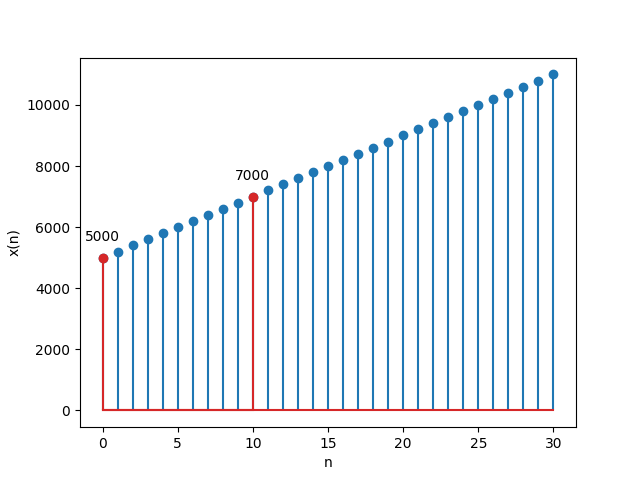
\includegraphics[width=\columnwidth]{ncert-maths/10/5/2/19/figs/10_5_2_19.png}
    \caption{Plot of $x(n)$ vs $n$. See \tabref{tab:math_10_5_2_19} for details.}
    \label{fig:math_10_5_2_19}
\end{figure}
Let Z-transform of $x(n)$ be $X(z)$.
\begin{align}
X(z) &= \frac{x(0)}{1 - z^{-1}} + \frac{dz^{-1}}{(1 - z^{-1})^2} \quad |z| > 1
\end{align}
Using the values from \tabref{tab:math_10_5_2_19}:
\begin{align}
X(z) &= \frac{5000}{1 - z^{-1}} + \frac{200z^{-1}}{(1 - z^{-1})^2} \quad |z| > 1
\end{align}
%\end{document}


\item Consider the sequence whose $n^\text{th}$ term is given by \(2^n\). Find the first 6 terms of this sequence.

\solution

%\iffalse
\let\negmedspace\undefined
\let\negthickspace\undefined
\documentclass[journal,12pt,onecolumn]{IEEEtran}
\usepackage{cite}
\usepackage{amsmath,amssymb,amsfonts,amsthm}
%\usepackage{algorithmic}
\usepackage{graphicx}
\usepackage{textcomp}
\usepackage{array}
\usepackage{xcolor}
\usepackage{txfonts}
\usepackage{listings}
\usepackage{enumitem}
\usepackage{mathtools}
\usepackage{gensymb}
\usepackage[breaklinks=true]{hyperref}
\usepackage{tkz-euclide} % loads  TikZ and tkz-base
\usepackage{listings}
\usepackage{float}



\newtheorem{theorem}{Theorem}[section]
\newtheorem{problem}{Problem}
\newtheorem{proposition}{Proposition}[section]
\newtheorem{lemma}{Lemma}[section]
\newtheorem{corollary}[theorem]{Corollary}
\newtheorem{example}{Example}[section]
\newtheorem{definition}[problem]{Definition}
%\newtheorem{thm}{Theorem}[section] 
%\newtheorem{defn}[thm]{Definition}
%\newtheorem{algorithm}{Algorithm}[section]
%\newtheorem{cor}{Corollary}
\newcommand{\BEQA}{\begin{eqnarray}}
\newcommand{\EEQA}{\end{eqnarray}}
\newcommand{\define}{\stackrel{\triangle}{=}}
\theoremstyle{remark}
\newtheorem{rem}{Remark}
%\bibliographystyle{ieeetr}
\begin{document}
%
\providecommand{\pr}[1]{\ensuremath{\Pr\left(#1\right)}}
\providecommand{\prt}[2]{\ensuremath{p_{#1}^{\left(#2\right)} }}        % own macro for this question
\providecommand{\qfunc}[1]{\ensuremath{Q\left(#1\right)}}
\providecommand{\sbrak}[1]{\ensuremath{{}\left[#1\right]}}
\providecommand{\lsbrak}[1]{\ensuremath{{}\left[#1\right.}}
\providecommand{\rsbrak}[1]{\ensuremath{{}\left.#1\right]}}
\providecommand{\brak}[1]{\ensuremath{\left(#1\right)}}
\providecommand{\lbrak}[1]{\ensuremath{\left(#1\right.}}
\providecommand{\rbrak}[1]{\ensuremath{\left.#1\right)}}
\providecommand{\cbrak}[1]{\ensuremath{\left\{#1\right\}}}
\providecommand{\lcbrak}[1]{\ensuremath{\left\{#1\right.}}
\providecommand{\rcbrak}[1]{\ensuremath{\left.#1\right\}}}
\newcommand{\sgn}{\mathop{\mathrm{sgn}}}
\providecommand{\abs}[1]{\left\vert#1\right\vert}
\providecommand{\res}[1]{\Res\displaylimits_{#1}} 
\providecommand{\norm}[1]{\left\lVert#1\right\rVert}
%\providecommand{\norm}[1]{\lVert#1\rVert}
\providecommand{\mtx}[1]{\mathbf{#1}}
\providecommand{\mean}[1]{E\left[ #1 \right]}
\providecommand{\cond}[2]{#1\middle|#2}
\providecommand{\fourier}{\overset{\mathcal{F}}{ \rightleftharpoons}}
\newenvironment{amatrix}[1]{%
  \left(\begin{array}{@{}*{#1}{c}|c@{}}
}{%
  \end{array}\right)
}
%\providecommand{\hilbert}{\overset{\mathcal{H}}{ \rightleftharpoons}}
%\providecommand{\system}{\overset{\mathcal{H}}{ \longleftrightarrow}}
	%\newcommand{\solution}[2]{\textbf{Solution:}{#1}}
\newcommand{\solution}{\noindent \textbf{Solution: }}
\newcommand{\cosec}{\,\text{cosec}\,}
\providecommand{\dec}[2]{\ensuremath{\overset{#1}{\underset{#2}{\gtrless}}}}
\newcommand{\myvec}[1]{\ensuremath{\begin{pmatrix}#1\end{pmatrix}}}
\newcommand{\mydet}[1]{\ensuremath{\begin{vmatrix}#1\end{vmatrix}}}
\newcommand{\myaugvec}[2]{\ensuremath{\begin{amatrix}{#1}#2\end{amatrix}}}
\providecommand{\rank}{\text{rank}}
\providecommand{\pr}[1]{\ensuremath{\Pr\left(#1\right)}}
\providecommand{\qfunc}[1]{\ensuremath{Q\left(#1\right)}}
	\newcommand*{\permcomb}[4][0mu]{{{}^{#3}\mkern#1#2_{#4}}}
\newcommand*{\perm}[1][-3mu]{\permcomb[#1]{P}}
\newcommand*{\comb}[1][-1mu]{\permcomb[#1]{C}}
\providecommand{\qfunc}[1]{\ensuremath{Q\left(#1\right)}}
\providecommand{\gauss}[2]{\mathcal{N}\ensuremath{\left(#1,#2\right)}}
\providecommand{\diff}[2]{\ensuremath{\frac{d{#1}}{d{#2}}}}
\providecommand{\myceil}[1]{\left \lceil #1 \right \rceil }
\newcommand\figref{Fig.~\ref}
\newcommand\tabref{Table~\ref}
\newcommand{\sinc}{\,\text{sinc}\,}
\newcommand{\rect}{\,\text{rect}\,}
%%
%	%\newcommand{\solution}[2]{\textbf{Solution:}{#1}}
%\newcommand{\solution}{\noindent \textbf{Solution: }}
%\newcommand{\cosec}{\,\text{cosec}\,}
%\numberwithin{equation}{section}
%\numberwithin{equation}{subsection}
%\numberwithin{problem}{section}
%\numberwithin{definition}{section}
%\makeatletter
%\@addtoreset{figure}{problem}
%\makeatother

%\let\StandardTheFigure\thefigure
\let\vec\mathbf

\bibliographystyle{IEEEtran}





\bigskip

%\renewcommand{\thefigure}{\theenumi}
%\renewcommand{\thetable}{\theenumi}
%\renewcommand{\theequation}{\theenumi}

Q: Consider the sequence whose $n^\text{th}$ term is given by \(2^n\). Find the first 6 terms of this sequence.

\solution

\begin{table}[!ht]
    \centering
        \begin{table}[ht]
    \centering
    \begin{tabular}{|c|c|c|}
        \hline
        Parameter & Value & Description \\
        \hline
        $x(0)$ & 5 & First term of AP \\
        $d$ & 1.75 & Common difference of AP \\
        $x(n)$ & 20.75 & $n^{th}$ term of AP \\
        \hline
    \end{tabular}
    \vspace{2mm}
    \caption{Parameter List}
    \label{tab:simple.10.5.2.20}
\end{table}

    \caption{input parameters}
    \label{tab:11_9_1_3}
\end{table}
%\fi
\begin{align}
X(Z) &= \frac {1}{1 - 2  z^{-1} } \quad \abs{z}>\abs{2}
\end{align}

\begin{figure}[H]
    \centering
    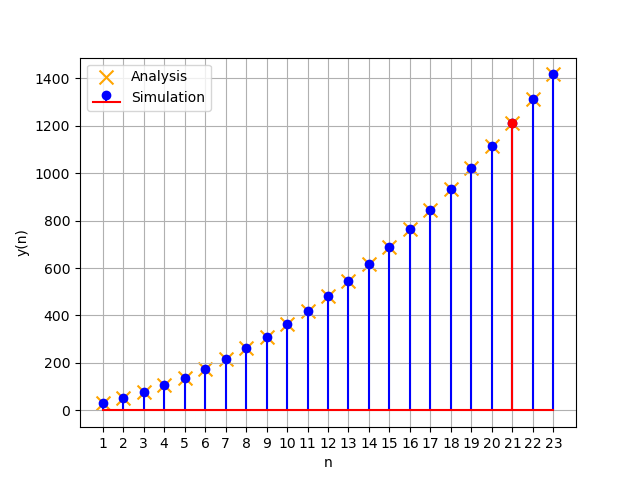
\includegraphics{figs/fig1.png}
    \caption{Six terms of given sequence}
    \label{fig:11_9_1_3 }
\end{figure}

\end{document}


\item If the sum of first 7 terms of an AP is 49 and that of 17 terms is 289, find the sum of first n terms.

\solution

\iffalse
\let\negmedspace\undefined
\let\negthickspace\undefined
\documentclass[journal,12pt,twocolumn]{IEEEtran}
\usepackage{cite}
\usepackage{amsmath,amssymb,amsfonts,amsthm}
\usepackage{algorithmic}
\usepackage{graphicx}
\usepackage{textcomp}
\usepackage{xcolor}
\usepackage{txfonts}
\usepackage{listings}
\usepackage{enumitem}
\usepackage{mathtools}
\usepackage{gensymb}
\usepackage{comment}
\usepackage[breaklinks=true]{hyperref}
\usepackage{tkz-euclide} 
\usepackage{listings}
\usepackage{gvv}                                        
\def\inputGnumericTable{}                                 
\usepackage[latin1]{inputenc}                                
\usepackage{color}                                            
\usepackage{array}                                            
\usepackage{longtable}                                       
\usepackage{calc}                                             
\usepackage{multirow}                                         
\usepackage{hhline}                                           
\usepackage{ifthen}                                           
\usepackage{lscape}
\newtheorem{theorem}{Theorem}[section]
\newtheorem{problem}{Problem}
\newtheorem{proposition}{Proposition}[section]
\newtheorem{lemma}{Lemma}[section]
\newtheorem{corollary}[theorem]{Corollary}
\newtheorem{example}{Example}[section]
\newtheorem{definition}[problem]{Definition}
\newcommand{\BEQA}{\begin{eqnarray}}
\newcommand{\EEQA}{\end{eqnarray}}
\newcommand{\define}{\stackrel{\triangle}{=}}
\theoremstyle{remark}
\newtheorem{rem}{Remark}
\begin{document}

\bibliographystyle{IEEEtran}
\vspace{3cm}

\title{10.5.3.9}
\author{EE23BTECH11063 - Vemula Siddhartha
}
\maketitle
\newpage
\bigskip

\renewcommand{\thefigure}{\theenumi}
\renewcommand{\thetable}{\theenumi}
\textbf{Question}:\\
If the sum of first 7 terms of an AP is 49 and that of 17 terms is 289, find the sum of
first n terms.
\\
\textbf{Solution: }
\fi
\begin{table}[h!]    
  \centering
  \begin{tabular}[12pt]{ |c| c|}
    \hline
    \textbf{Variable} & \textbf{Description}\\ 
    \hline
    $x\brak{0}$ & First term of the AP \\
    \hline 
    $d$ & Common difference of the AP\\
    \hline
    $y\brak{n}$ & Sum of $n+1$ terms of the AP\\
    \hline
    $x\brak{n}$ & General term\\
    \hline   
    \end{tabular}
  \caption{Variables Used}
  \label{tab10.5.3.9.1}
\end{table}
\begin{align}
y\brak{n}&=\frac{n+1}{2}\,\brak{2x\brak{0}+nd}\,u\brak{n}\label{eq10.5.3.9.1}\\
y\brak{6}&=49\\
y\brak{16}&=289
\end{align}
Then,
\begin{align}
x\brak{0}+3d&=7\label{eq10.5.3.9.2}\\
x\brak{0}+8d&=17 \label{eq10.5.3.9.3}
\end{align}
From  equations \ref{eq10.5.3.9.2} and \ref{eq10.5.3.9.3}, the augmented matrix is:
\begin{align}
 \myvec{
   1 & 3 & 7
   \\
   1 & 8 & 17
 }
 \xleftrightarrow[]{R_2 \leftarrow {R_2-R_1}}
 \myvec{
   1 & 3 & 7
   \\
   0 & 5 & 10
 }
 \\
 \xleftrightarrow[]{R_1 \leftarrow {R_1-\frac{3}{5}R_2}}
 \myvec{
   1 & 0 & 1
   \\
   0 & 5 & 10
 }
 \\
 \xleftrightarrow[]{R_2 \leftarrow \frac{R_2}{5}}
 \myvec{
   1 & 0 & 1
   \\
   0 & 1 & 2
 }
 \\
 \implies \myvec{
   x\brak{0}
   \\
   d
 }
 =
 \myvec{
   1
   \\
   2
 }
\end{align}
\begin{align}
    x\brak{n}&= \brak{1+2n}u\brak{n}\\
    X\brak{z}&=\frac{1}{1-z^{-1}}+\frac{2z^{-1}}{\brak{1-z^{-1}}^2}\;\;\cbrak{z\in\mathbb{C}: |z|>1}
\end{align}
\begin{align}
   y\brak{n}&=x\brak{n}*u\brak{n}\\
   Y\brak{z}&=X\brak{z}\,U\brak{z}\\
   \implies Y\brak{z}&=\brak{\frac{1}{1-z^{-1}}+\frac{2z^{-1}}{\brak{1-z^{-1}}^2}}\brak{\frac{1}{1-z^{-1}}}\\
   &=\frac{1}{\brak{1-z^{-1}}^2}+\frac{2z^{-1}}{\brak{1-z^{-1}}^3}\\
   \brak{n+1}u\brak{n}&\system{Z}\frac{1}{\brak{1-z^{-1}}^2}\cbrak{z\in\mathbb{C}: |z|>1}\\
   n\brak{\brak{n+1}u\brak{n}}&\system{Z}\frac{2z^{-1}}{\brak{1-z^{-1}}^3}\cbrak{z\in\mathbb{C}: |z|>1}
\end{align}
   From equations \eqref{eq:uzder-shift} and \eqref{eq:uzder-der}, taking the inverse Z Transform,
   \begin{align}
   y\brak{n}&=\brak{n+1}u\brak{n}+n\brak{\brak{n+1}u\brak{n}}\\
   \implies y\brak{n}&=\brak{n+1}^2\,u\brak{n}
\end{align}
\begin{figure}[h!]
   \centering
   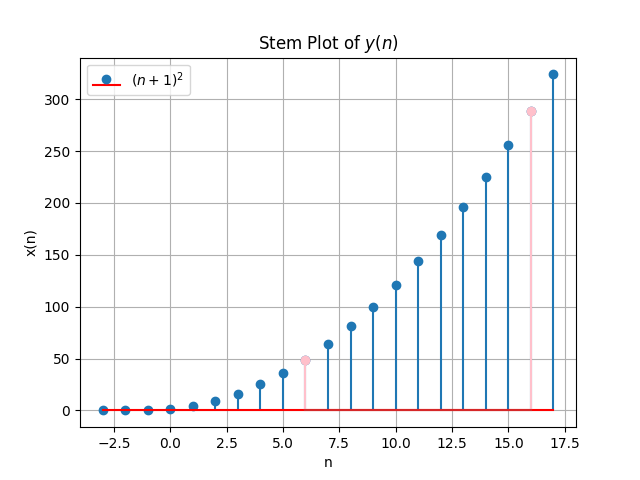
\includegraphics[width=1.1\linewidth]{ncert-maths/10/5/3/9/figs/Figure_1.png}
   \caption{Stem Plot of y\brak{n}}
   \label{stemplot}
\end{figure}  

\pagebreak

\item Write the first five terms of the sequence and obtain the corresponding series:\\
$a_1=a_2=2,$ $a_n=a_{n-1} -1,$ $n>2$\\
\solution
\iffalse
\let\negmedspace\undefined
\let\negthickspace\undefined
\documentclass[journal,12pt,twocolumn]{IEEEtran}
\usepackage{cite}
\usepackage{amsmath,amssymb,amsfonts,amsthm}
\usepackage{algorithmic}
\usepackage{graphicx}
\usepackage{textcomp}
\usepackage{xcolor}
\usepackage{txfonts}
\usepackage{listings}
\usepackage{enumitem}
\usepackage{mathtools}
\usepackage{float}
\usepackage{gensymb}
\usepackage{comment}
\usepackage[breaklinks=true]{hyperref}
\usepackage{tkz-euclide} 
\usepackage{listings}
\usepackage{gvv}                                        
\def\inputGnumericTable{}                                 
\usepackage[latin1]{inputenc}                                
\usepackage{color}                                            
\usepackage{array}                                            
\usepackage{longtable}                                       
\usepackage{calc}                                             
\usepackage{multirow}                                         
\usepackage{hhline}                                           
\usepackage{ifthen}                                           
\usepackage{lscape}
\usepackage{amsmath}
\newtheorem{theorem}{Theorem}[section]
\newtheorem{problem}{Problem}
\newtheorem{proposition}{Proposition}[section]
\newtheorem{lemma}{Lemma}[section]
\newtheorem{corollary}[theorem]{Corollary}
\newtheorem{example}{Example}[section]
\newtheorem{definition}[problem]{Definition}
\newcommand{\BEQA}{\begin{eqnarray}}
\newcommand{\EEQA}{\end{eqnarray}}
\newcommand{\define}{\stackrel{\triangle}{=}}
\theoremstyle{remark}
\newtheorem{rem}{Remark}
\begin{document}
\bibliographystyle{IEEEtran}
\title{NCERT 11.9.1.13Q}
\author{EE23BTECH11015 - DHANUSH V NAYAK$^{*}$% <-this % stops a space
}
\maketitle
\newpage
\bigskip
\renewcommand{\thefigure}{\arabic{figure}}
\renewcommand{\thetable}{\theenumi}
\textbf{Question:} Write the first five terms of each of the sequences in Exercises 11 to 13 and obtain the corresponding series:\\
$a_1=a_2=2,$\hspace{5pt} $a_n=a_{n-1} -1,$\hspace{5pt} $n>2$\\
\solution
\fi
\begin{table}[H]
    \centering
    \renewcommand\thetable{1}
    \setlength{\extrarowheight}{9pt}
    \resizebox{0.5\textwidth}{!}{
    \begin{tabular}{|c|c|c|}
    \hline
    \textbf{Parameter} & \textbf{Description} & \textbf{Value} \\ \hline
    $x\brak{0}$ & First term &2 \\ \hline
    $x\brak{1}$ & Second term &2 \\ \hline
    ROC & Region of convergence & $\left\{ z : \left|\sum_{n=-\infty}^{\infty} x(n)z^{-n}\right| < \infty \vphantom {\brak{{0.3pt}}}\right\}$ \\ \hline 
    $x(n)$ & General term & $x(n) = 
    \begin{cases}
        ? & ; n \geq 0 \\
        0 & ; n < 0 \\
    \end{cases}$ \\ \hline
    \end{tabular}}
    \caption{Parameter Table}
    \label{tab:11.9.1.13}
    \end{table}
\begin{align}
    x\brak{n} - x\brak{n-1} &= 2u\brak{n}-2u\brak{n-1}-u\brak{n-2}\label{eq:11.9.1.13.1}\\
X\brak{z}- z^{-1}X\brak{z} &= \frac{2}{\brak{1-z^{-1}}} - \frac{z^{-2}}{\brak{1-z^{-1}}}- \frac{2z^{-1}}{\brak{1-z^{-1}}}\\
    X\brak{z} &= \frac{2-2z^{-1}-z^{-2}}{\brak{1-z^{-1}}^2}  ,   \abs{z} >1
\end{align}
Using partial fractions
\begin{align}
    X\brak{z} &= \frac{2z^{-1}}{\brak{1-z^{-1}}} - \frac{z^{-2}}{\brak{1-z^{-1}}^2} + 2\label{eq:11.9.1.13.5}
\end{align}
Taking inverse $Z$-transform by result of equation \eqref{eq:11.9.5.26.9} in equation \eqref{eq:11.9.1.13.5}:
\begin{align}
    x\brak{n} &= 2u\brak{n}+\brak{1-n}u\brak{n-1}\label{eq:11.9.1.13.6}
\end{align}
\begin{figure}[H]
    \centering
    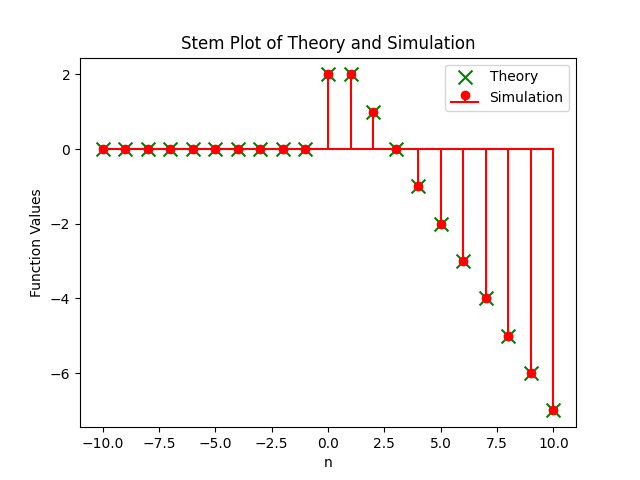
\includegraphics[width=1\columnwidth]{ncert-maths/11/9/1/13/figs/Theory_vs_Simulation.png}
    \caption{Comparison of Theory and Simulated Values}
    \label{fig:11.9.1.13.1}
\end{figure}
From the figure\figref{fig:11.9.1.13.1} we can see that the theoretical and simulated values overlap. 
%\end{document}

\pagebreak
\item Insert two numbers between 3 and 81 so that the resulting sequence is G.P.\\

\solution
\iffalse
\let\negmedspace\undefined
\let\negthickspace\undefined
\documentclass[journal,12pt,twocolumn]{IEEEtran}
\usepackage{cite}
\usepackage{amsmath,amssymb,amsfonts,amsthm}
\usepackage{algorithmic}
\usepackage{graphicx}
\usepackage{textcomp}
\usepackage{xcolor}
\usepackage{txfonts}
\usepackage{listings}
\usepackage{enumitem}
\usepackage{mathtools}
\usepackage{gensymb}
\usepackage{comment}
\usepackage[breaklinks=true]{hyperref}
\usepackage{tkz-euclide}
\usepackage{listings}
\usepackage{gvv}
\def\inputGnumericTable{}
\usepackage[latin1]{inputenc}
\usepackage{color}
\usepackage{array}
\usepackage{longtable}
\usepackage{calc}
\usepackage{multirow}
\usepackage{hhline}
\usepackage{ifthen}
\usepackage{lscape}

\newtheorem{theorem}{Theorem}[section]
\newtheorem{problem}{Problem}
\newtheorem{proposition}{Proposition}[section]
\newtheorem{lemma}{Lemma}[section]
\newtheorem{corollary}[theorem]{Corollary}
\newtheorem{example}{Example}[section]
\newtheorem{definition}[problem]{Definition}
\newcommand{\BEQA}{\begin{eqnarray}}
\newcommand{\EEQA}{\end{eqnarray}}
\newcommand{\define}{\stackrel{\triangle}{=}}
\theoremstyle{remark}
\newtheorem{rem}{Remark}
\begin{document}

\bibliographystyle{IEEEtran}
\vspace{3cm}

\title{NCERT Discrete 11.9.3 -26}
\author{EE23BTECH11057 - Shakunaveti Sai Sri Ram Varun$^{}$% &lt;-this % stops a space
}
\maketitle
\newpage
\bigskip
\vspace{2cm}
\textbf{Question: }
Insert two numbers between 3 and 81 so that the resulting sequence is G.P.\\
\textbf{Solution}:
\fi
\begin{table}[htbp] 
\centering
\begin{tabular}{|c|c|c|}
    \hline
    \textbf{Parameter} & \textbf{Description} & \textbf{Value} \\
    \hline
    $x\brak{0}$ & First term of G.P. & 3 \\
    \hline
    $x\brak{3}$ & Fourth term of G.P. & 81 \\
    \hline
    $r$ & common ratio of G.P. & r \\
    \hline
\end{tabular}



\caption{input values}
\label{tab: Table 11.9.3.26.15}
\end{table}
\begin{enumerate}
\item 
\begin{align}
x\brak{n}=x\brak{0}r^{n}
\end{align}
from the values in \tabref{tab: Table 11.9.3.26.15}
\begin{align}
%x(0)&=3\\
%x(3)&=81\\
\frac{x\brak{0}r^3}{x\brak{0}}&=27\\
r&=3
\end{align}
$ \therefore $ Required numbers are 9 and 27.
\item 
\begin{align}
x\brak{n} &= 3^{n+1}u\brak{n} \label{eq:11.9.3.26.1}\\
X\brak{z} &= \frac{3}{1-3z^{-1}} \quad |z|>3 \label{eq:11.9.3.26.2}
\end{align}
\begin{figure}[h!]
    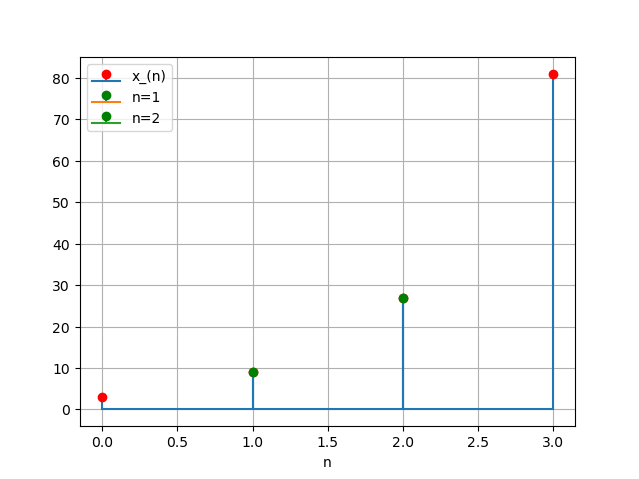
\includegraphics[width = \columnwidth]{ncert-maths/11/9/3/26/figs/Figure_1.png}
    \caption{Graph of $ x\brak{n}$ }
    \label{fig: 11.9.3.26.17}
\end{figure}
\end{enumerate}


\end{enumerate}
